\chapter{Конструкторский раздел}

В данном разделе представлены описание работы алгоритма; описание структур данных, используемых в алгоритме; описание способа тестирования; приведена оценка памяти для хранения данных и структура программного обеспечения.

\section{Описание работы алгоритмов}
На рисунке \ref{png:full_search} представлена схема алгоритма полного перебора поиска в словаре.
\begin{figure}[H]
	\centering{
		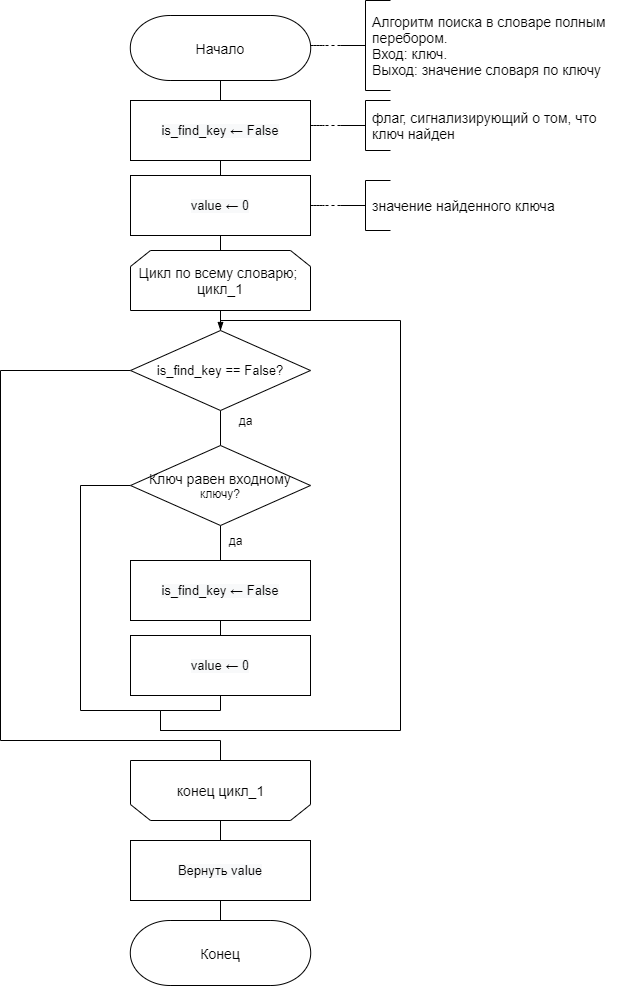
\includegraphics[scale=0.6]{../../../../../../../msys64/home/Лев/bmstu_sem_5_aa/lab_07/report/diagrams/full_search}
		\caption{Схема алгоритма полного перебора в словаре.}
		\label{png:full_search}
			}
\end{figure}

На рисунке \ref{png:binary_search} представлена схема алгоритма бинарного поиска в словаре.
\begin{figure}[H]
	\centering{
		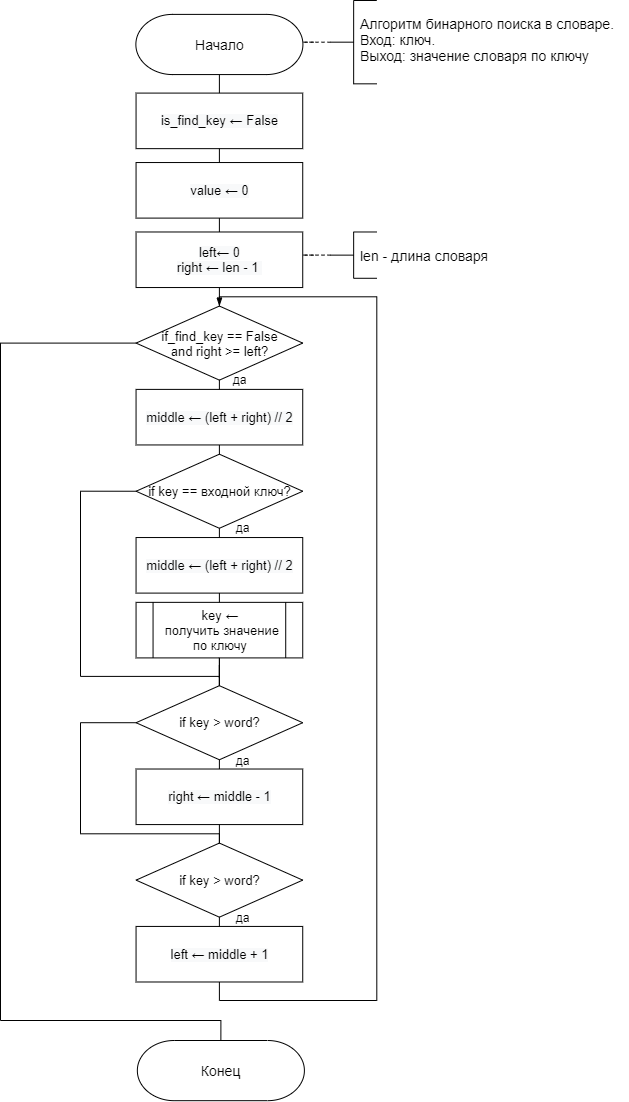
\includegraphics[scale=0.6]{../../../../../../../msys64/home/Лев/bmstu_sem_5_aa/lab_07/report/diagrams/binary_search}
		\caption{Схема алгоритма бинарного поиска в словаре.}
		\label{png:binary_search}
	}
\end{figure}

\newpage
На рисунке \ref{png:segment_search} представлена схема алгоритма поиска сегментами с бинарным поиском внутри в словаре.
\begin{figure}[H]
	\centering{
		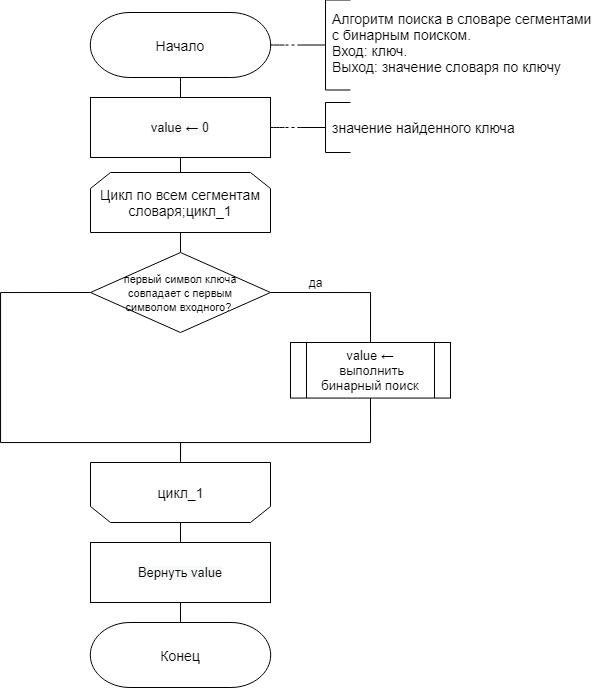
\includegraphics[scale=0.6]{../../../../../../../msys64/home/Лев/bmstu_sem_5_aa/lab_07/report/diagrams/segment_search}
		\caption{Схема алгоритма поиска сегментами в словаре.}
		\label{png:segment_search}
	}
\end{figure}

\section{Описание структур данных}
Словарь представлен следующей структурой данных:
\begin{itemize}
	\item Dictionary - тип данных, описывающих ассоциативный массив с ключами типа string.
\end{itemize}

\section{Описание способа тестирования и выделенных классов эквивалентности}
Тестирование программного обеспечения будет выполнено, используя матрицу смежности, а также набор регулируемых параметров. Матрица является симметричной, диагональные элементы равны нулю.

В качестве классов эквивалентности можно выделить стоимость пути между городами: порядка 50-100 и 500-1000 условных единиц.

\section{Оценка памяти для хранения данных}

Расчет памяти, используемой для хранения словаря, производится по формуле \ref{math:mem-nonseg}.
\begin{equation}\label{math:mem-nonseg}
	M_{dict} = N \cdot (|char| \cdot |key_i| + |int|)
\end{equation}
где $N$ -- количество слов в словаре, $|char|$ -- размер переменной типа <<символ>>, $|key_i|$ -- длина ключа, $|int|$ --  размер переменной типа <<целое>>.
Расчет памяти, используемой под сегментированный массив, вычисляется по формуле \ref{math:mem-seg}.
\begin{equation}\label{math:mem-seg}
	M_{seg-dict} = S \cdot M_{dict}
\end{equation}
Где $S$ -- количество сегментов.

\section{Структура программного обеспечения}
В качестве парадигмы было использованы структурное программирование в сочетании с объектно-ориентированным. Программное обеспечение состоит из нескольких модулей:
\begin{itemize}
	\item main - главный модуль, который выполняет вызов функций решения поиска в  словаре;
	\item dictionary - модуль, содержащий необходимые структуры данных и реализацию методов поиска в словаре;
	\item menu - модуль, содержащий меню для консольного вывода на экран;
	\item cities - модуль, описывающий необходимые структуры и функции для создания массива городов;
	\item word - модуль, необходимый для вывода результата найденного значения (или сообщение об ошибке).
\end{itemize}

\section{Выделение классов эквивалентности}

Для тестирования программного обеспечения выделены следующие случаи:
\begin{itemize}
	\item искомый ключ присутствует в словаре, в текстовом файле располагается не в первой и не в последней строке;
	\item искомый ключ присутствует в словаре, в текстовом файле располагается в последней строке;
	\item искомый ключ присутствует в словаре, в текстовом файле располагается в первой строке;
	\item искомый ключ не присутствует в словаре.
\end{itemize}

\section{Вывод}
Были описаны алгоритмы полного перебора и муравьиным методом. Были описаны структуры данных, необходимые для реализации программного обеспечения. Были выделены классы эквивалентности и описан способ тестирования.